
\documentclass{article}
\usepackage[utf8]{inputenc}
\usepackage[spanish]{babel}
\usepackage{graphicx}
\usepackage{geometry}
\usepackage{enumerate}
\usepackage{titlesec}
\usepackage{float}

\geometry{letterpaper, margin = 1.5cm}

%Datos de la Portada
\title{Herrramientas Computacionales \\ Practica 1}
\author{Medina Martinez Jonathan Jason \\ 2023640061}
\date{22 de febrero de 2023}

\begin{document} %Inicio del Documento

\fontsize{16}{18}\selectfont

\begin{figure}[t] %Logos Portada


\includegraphics[width=2.5 cm]{Logo1.jpeg}
\hfill

\includegraphics[width=3 cm]{Logo2.png}

\end{figure}

\maketitle %Titulo Portada
\newpage

\tableofcontents %Indice
\newpage

\section{Objetivo}

Conocer el ambiente del lenguaje de programacion en C, el manejo de entradas y salidas y operaciones basicas.
\section{Introducción}
En esta practica se creara un programa que solicite informacion al usuario y despues la imprima en pantalla, ademas de crear por la terminal los archivos .o, .i y el ejecutable (.exe) desde la terminal.
\newpage

\section{Desarrollo}
\subsection{Creacion del Programa}
Para la creacion de este programa se declararon las variables al principio del mismo para que este almacene dichas variables desde el comienzo del mismo.

Este programa solicita al usuario su nombre y lo almacenma en la variable del mismo nombre, despues solicita  la usuario su edad y la almacena en la variable del mismo nombre, consecuente a esto solicita la estatura al usuario en metros almacenandola en la variable estatura.

Calcula el año de nacimiento restandole la edad al año en curso, Imprime en pantalla los datos recabados y calculados siendo estos el nombre, la edad, el año de nacimiento y la estatura, finalizando el programa.

\begin{figure}[H]
    \centering
    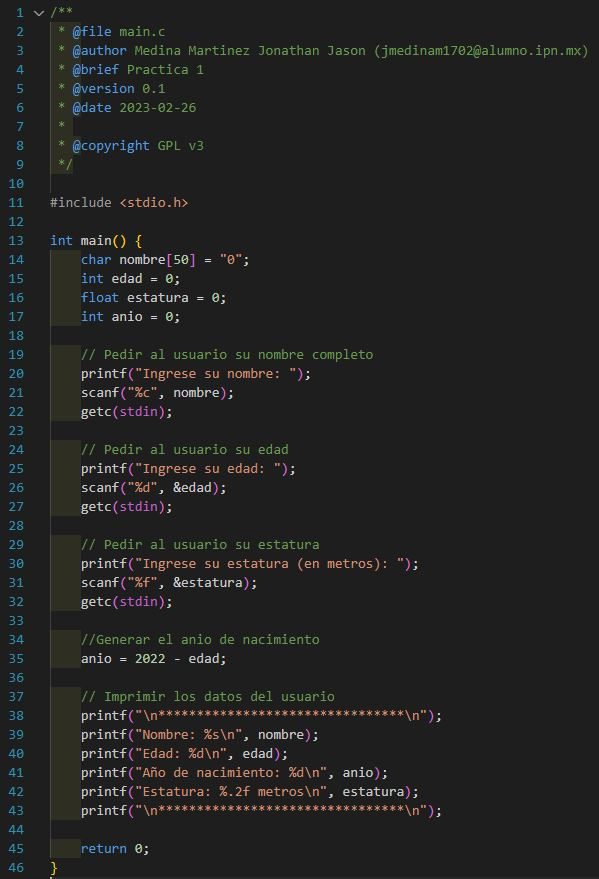
\includegraphics[height = 17cm]{Codigo.jpg}
\end{figure}
\subsubsection{Creacion de los archivos desde la terminal}

Para la cracion de los archivos se escribiran los siguientes comandos en la terminal de visual studio code:

\begin{enumerate}

    \item gcc -E main.c -o main.i
    \item gcc -c main.i -o main.o
    \item ar -cvr main.a main.o
    \item gcc -Wall main.o -L -lmain -o main
    
\end{enumerate}

\begin{figure}[H]
    \centering
    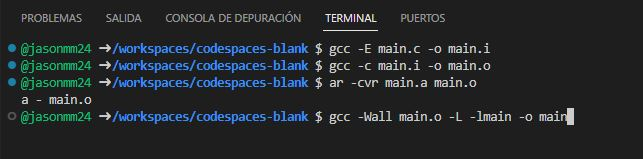
\includegraphics[width = 18cm]{Comandos.jpg}
\end{figure}

Generando asi los siguientes archivos:

\begin{figure}[H]
    \centering
    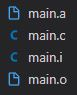
\includegraphics[height = 6cm]{Archivos.jpg}
\end{figure}

\newpage

\section{Resultados}

Al ejecutar el programa se obtiene lo siguiente:

\begin{figure}[H]
    \centering
    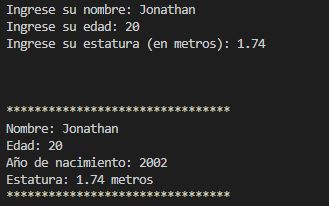
\includegraphics[width = 10cm]{Programa.jpg}
\end{figure}

\newpage

\section{Conclusiones}

Los diferentes tipos de variables nos permiten tener y almacenar diferentes tipos de datos por ejemplo una variable "int" nos permite almacenar datos numericos de tiupo entero, una variable "char" nos permite guardar datos alfanumericos y la variable "float" nos permite guardar datos con decimales.

\newpage

\section{Referencias}

\textit{J., & J. (s. f.). 2023-2/main.c at main · j0z3ph/2023-2. GitHub. https://github.com/j0z3ph/2023-2/blob/main/IntrProg/C4/main.c}

\end{document}